\documentclass[a4paper,12pt]{article}
\usepackage{graphicx}
\graphicspath{ {../results/} }

\begin{document}
\pagestyle{headings}
\markright{Christopher S. Sidell csidell1@umbc.edu JZ28610 -- CMSC471 Proj2}

Given the following equation:

\begin{equation}
z = \frac{sin(x^2 + 3y^2)}{0.1+r^2}
+ (x^2 + 5y^2) * \frac{e^{1-r^2}}{2},
r = \sqrt{x^2+y^2}
\end{equation}

The following three algorithms were used to optimize and find the maximum of the function. Hill climbing from position x = 0.0 and y = 0.0. Then hill climbing with random restarts between -10 and 10 for about 20 times. The third test is simulated annealing with the probability function of $ e^{\frac{new-current}{temperature}} $

The results set:

\begin{center}
 \begin{tabular}{c c c}
 \hline
 Name & Highest Point & Time  \\ [0.5ex]
 \hline\hline
 Hill Climbing & 3.7262941710588473 & 0.008549928665161133  \\
 \hline
 Hill Climb with Restart & 0.5166799641198613 & 1.2141141891479492 \\
 \hline
 Simulated Annealing & 3.72795512062296 & 0.062128305435180664 \\
 \hline
\end{tabular}
\end{center}

The Hill Climbing without random restarts is just a lucky example as 0,0 has a good path straight to one of the highest points. Hill climbing with random restarts sometimes gets lucky and follows the path straight up or get stuck in a valley. The graphs generated below show a good example of how each path each iteration took.

Simulated Annealing more often than not will get the highest but takes slightly longer than the first test. Given the random restarts not always getting the highest and taking more time, a more accurate representation of the algorithm, hill climbing can be assumed that it will more often than not produce results that are not favorable. Whereas simulated annealing gives the highest within a shorter amount of time. So in a simple conclusion the simulated annealing algorithm is the best. Below you can see the example graphs in 3D space of the paths taken by each algorithm. Running the python code will result in an interactive version of the graph.

The graphs show three dimensions of x, y, and z (height). The colors are each iteration taken.

\centering
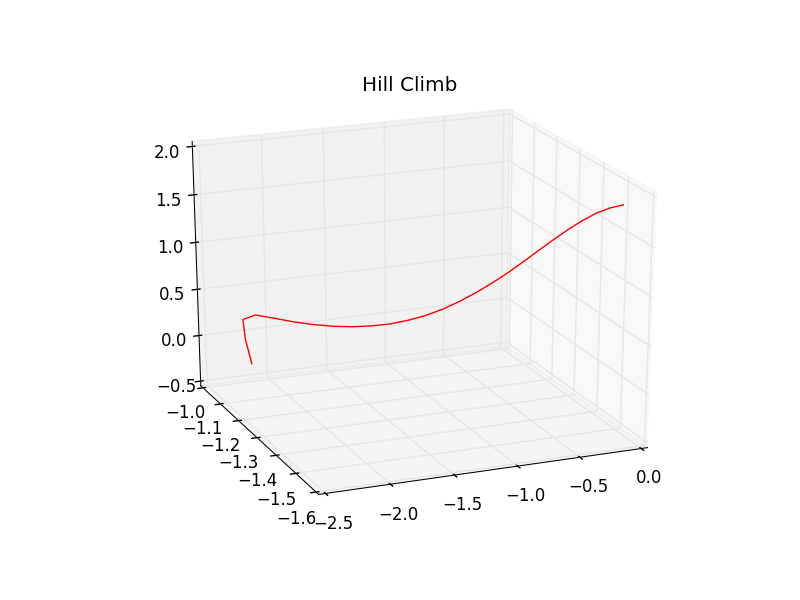
\includegraphics[scale=0.6]{hill_climb}
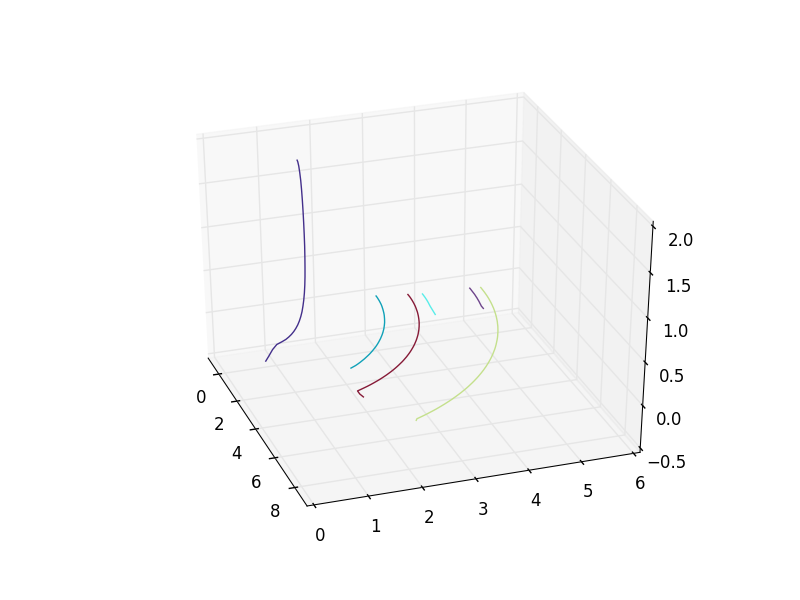
\includegraphics[scale=0.6]{hill_climb_random}
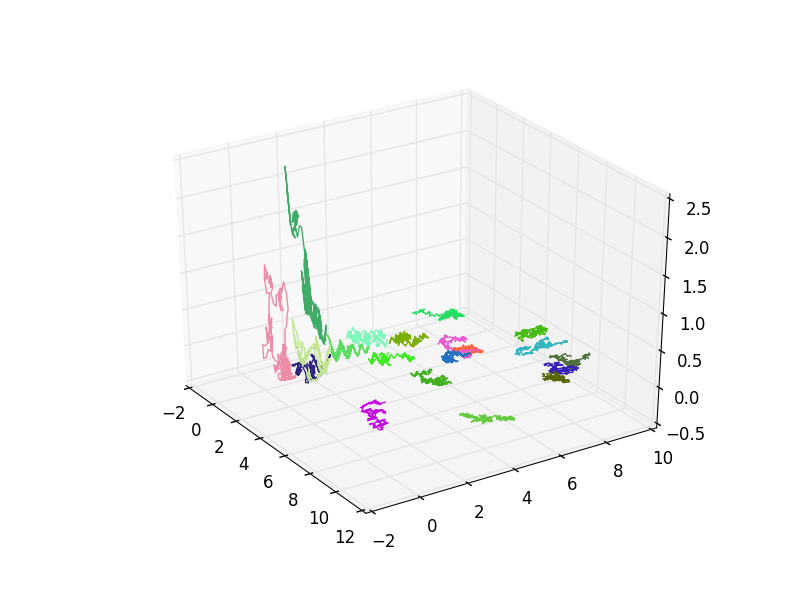
\includegraphics[scale=0.6]{simulated_annealing}

\end{document}